\chapter{Rischio geologico e adattamento ai cambiamenti climatici - Prof.ssa Claudia Romagnoli}
L'Antropocene ha una scala geologica molto breve rispetto ai cambiamenti climatici geologici naturali. Proterozoico prime fasi di vita in cui ufficialmente conosciamo di più. Fanerozoico è la fase più simile alla Terra attuale.
\begin{figure}[htpb]
    \centering
    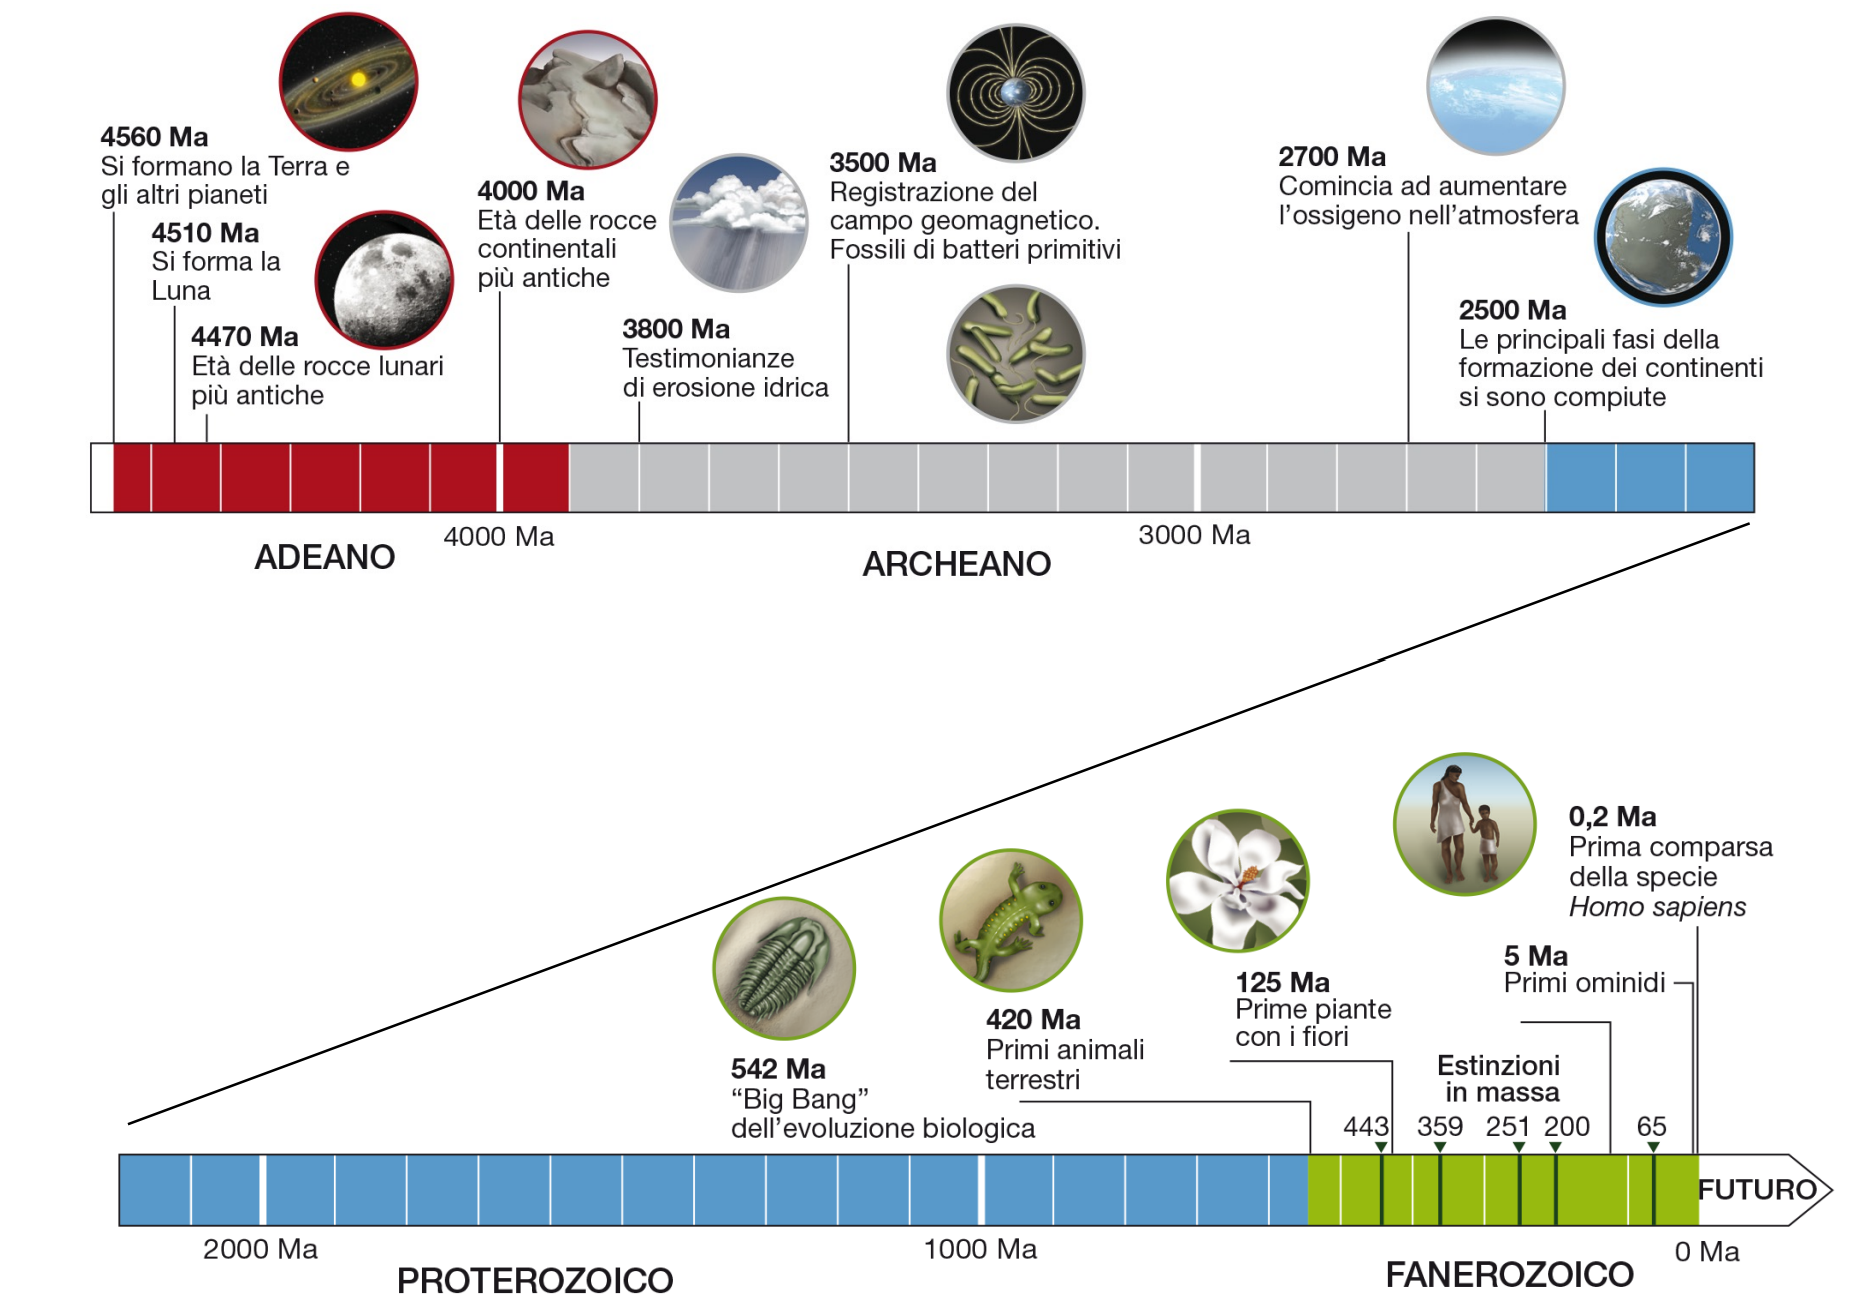
\includegraphics[width=0.5\linewidth]{uploads/scala.png}
    \caption{Linea del tempo}
    \label{fig:linea del tempo}
\end{figure}
Organismi più specializzati e meno adattabili sono le specie più a rischio di estinzione di massa. I primi ominidi compaiono negli ultimi anni. Prime forme di vita fine febbraio, prime forma di vita complessa fine ottobre, macro rettili - dicembre, l'uomo compare il 31/12 alle ore 23. Siamo arrivati negli ultimi secondi dell'evoluzione della terra. 20 000 anni fa l'ultimo evento di glaciazione massima. L'Olocene è una fase degli ultimi 10 000 anni che era di relativa stabilità climatica, momento di stallo delle fasi glaciali e interglaciali. 
\begin{figure}[htpb]
    \centering
    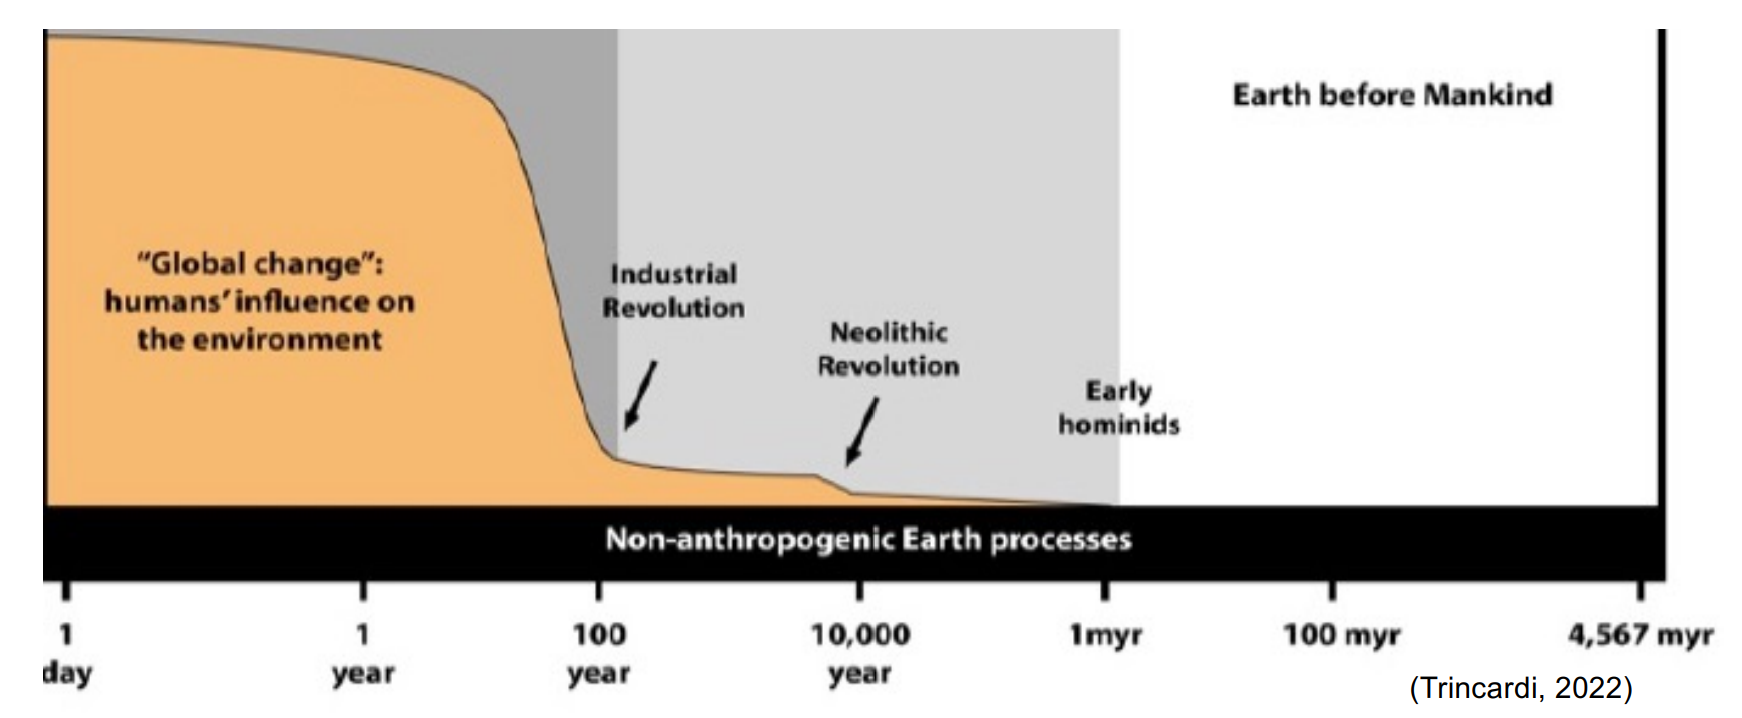
\includegraphics[width=0.5\linewidth]{uploads/Antropocene.png}
    \caption{Antropocene}
    \label{fig:antropocene}
\end{figure}
Antropocene (P. Crutzen, 2000): epoca geologica attuale, in cui l’ambiente terrestre,
nell’insieme delle sue caratteristiche fisiche, chimiche e biologiche, viene fortemente
condizionato su scala sia locale sia globale dagli effetti dell’azione umana, con
alterazioni sostanziali degli equilibri naturali.
\begin{figure}[htpb]
    \centering
    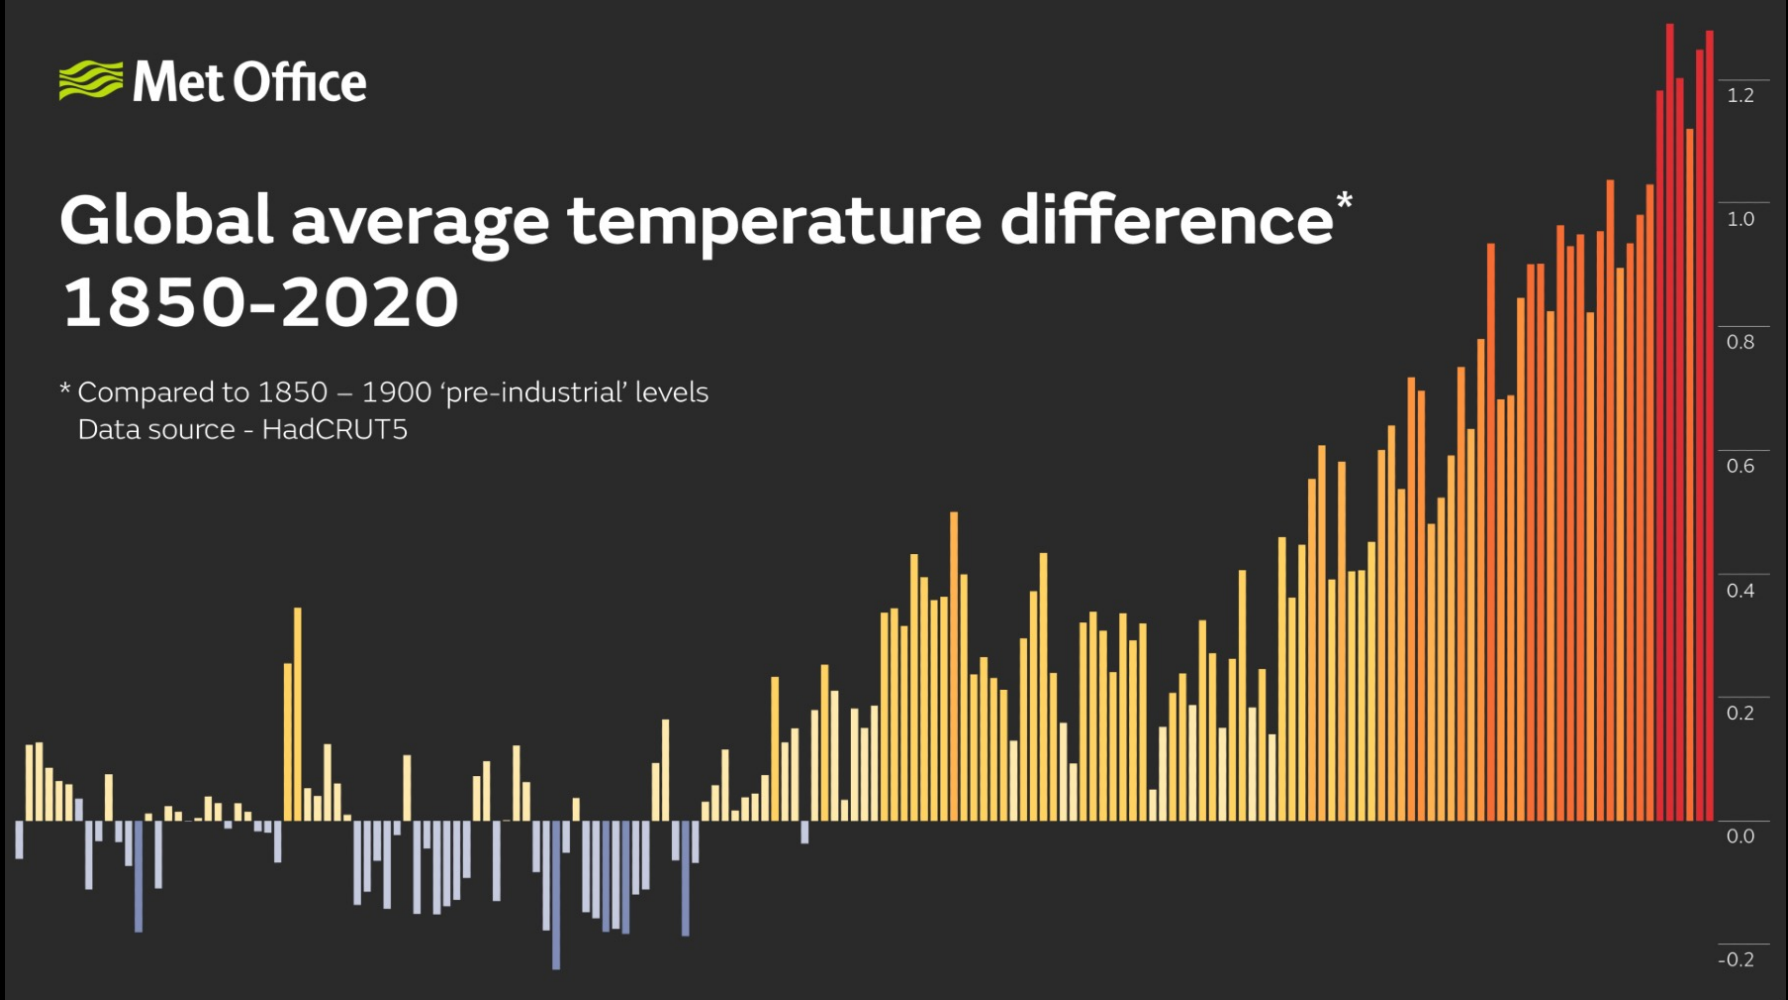
\includegraphics[width=0.5\linewidth]{uploads/global T.png}
\end{figure}
Vi sono componenti (e aree) del sistema climatico che risento più del cambiamento climatico, Il record isotopico dell’ossigeno registrato nei sedimenti
di mare profondo (tramite gusci di organismi fossili)
fornisce un dato indiretto, relativamente continuo e
sincrono, sul cambiamento delle masse glaciali e sulle
paleo-temperature degli oceani negli ultimi Ma. L’inizio della formazione di ghiacci nell’emisfero Nord (NHG) si ritiene iniziata
circa 2.7 Ma ago, probabilmente in connessione a vari processi geologici, quali
chiusura di passaggi oceanici e l’innalzamento della catena himalayana e
plateau tibetano, ed il conseguente cambio nello schema di circolazione
oceanica e dei venti, nella distribuzione del calore, albedo, ecc.
\begin{figure}[htpb]
    \centering
    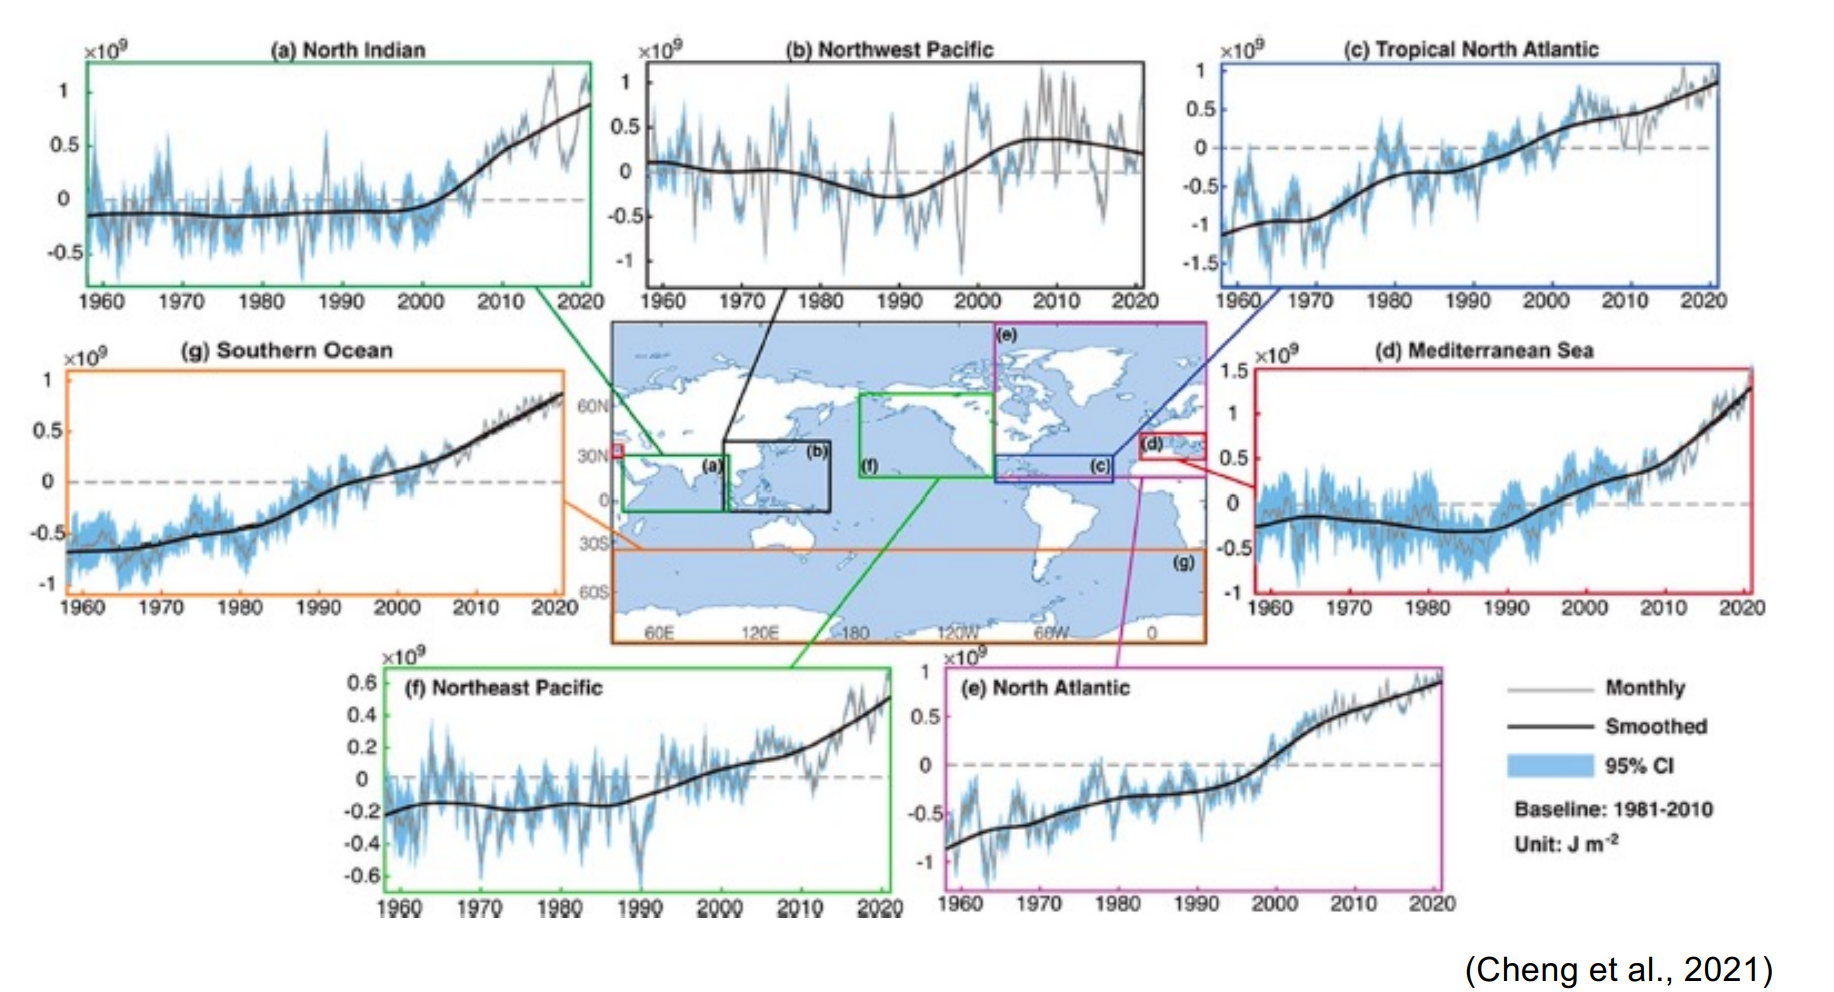
\includegraphics[width=0.5\linewidth]{uploads/cont.png}
    \caption{Come il contentuto in calore è variato dal 1960 al 2020 nei vari bacini.}
    \label{fig:cont bacini}
\end{figure}
In fig.\ref{fig:cont bacini} si vede come il Mediterraneo è un grande hotspot del cambiamento climatico. 
Siamo in grado di pensare a strategie che riducano l'impatto del cambiamento climatico? Mitigazione a adattamento.
Proxy sisgnifica dato indiretto: rapporto isotopico dell'ossigeno O18 o O16 strettamente legato alle paleotemperature conservato nei gusci carbonatici dei plankton. 
\begin{figure}[htpb]
    \centering
    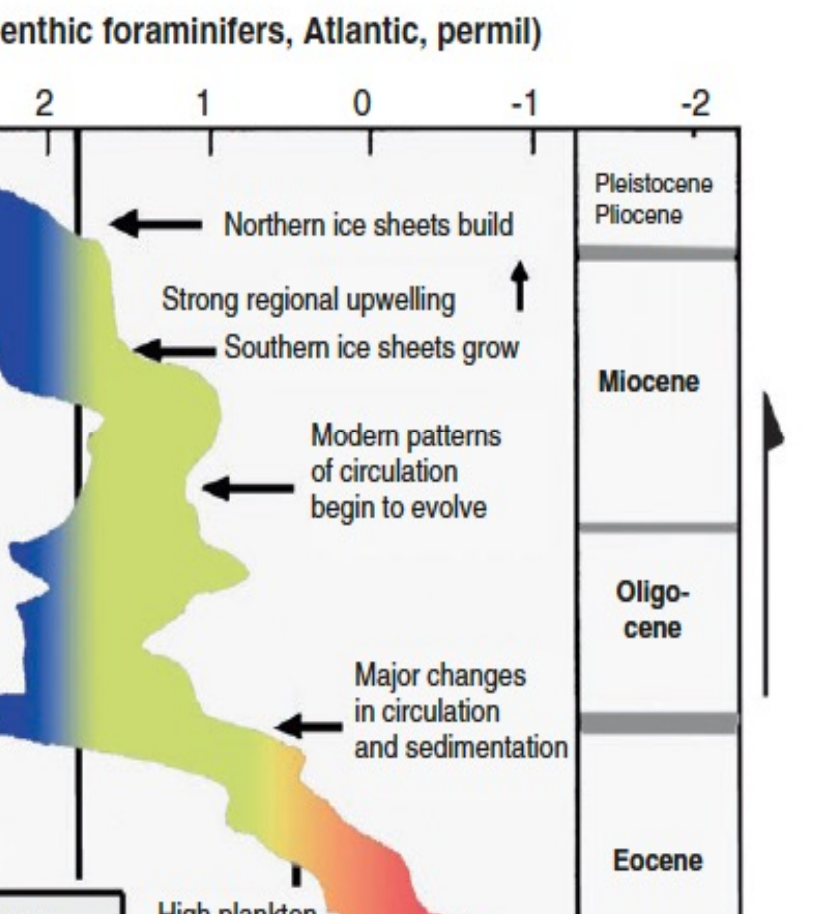
\includegraphics[width=0.5\linewidth]{uploads/deltaO18.png}
\end{figure}
caroteca
Negli interglaciali c'è rilascio del metano dai fondali marini. Cicli di Milankhovitch combinati assieme causano variazioni dell'insolazione sul pianeta fig.\ref{fig:insolazione}. 
\begin{figure}[htpb]
    \centering
    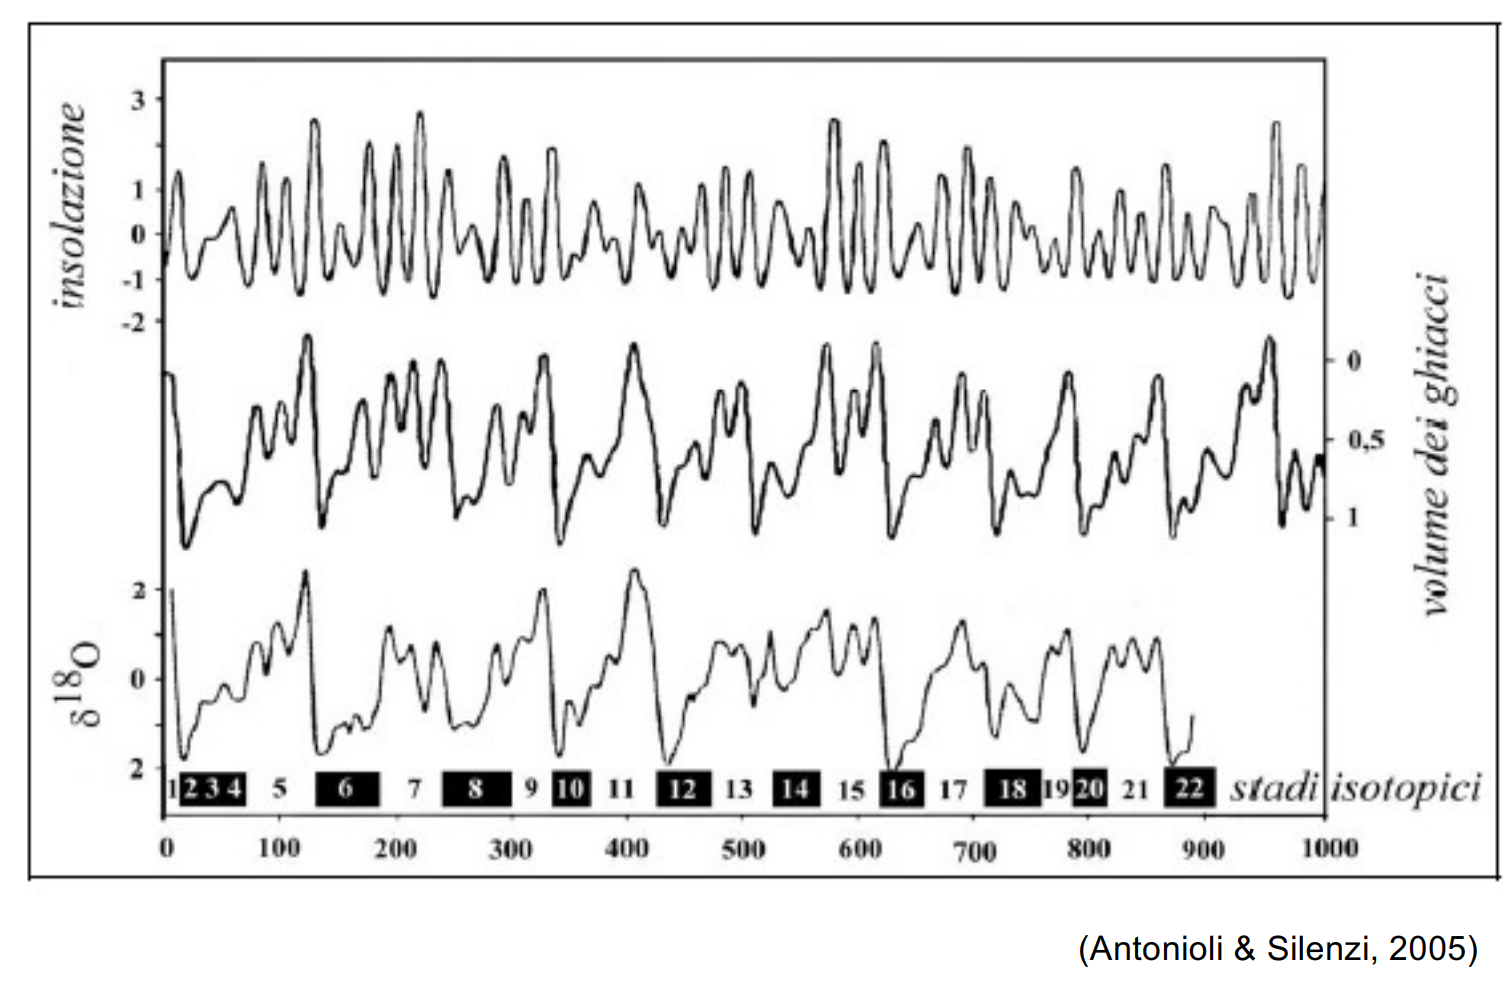
\includegraphics[width=0.5\linewidth]{uploads/insolazione.png}
    \label{fig:insolazione}
\end{figure}
stadi isotopici means neri glaciali, bianchi interglaciali ma questi cicli di paleotemperature non sono simmetrici. 
\begin{figure}[htpb]
    \centering
    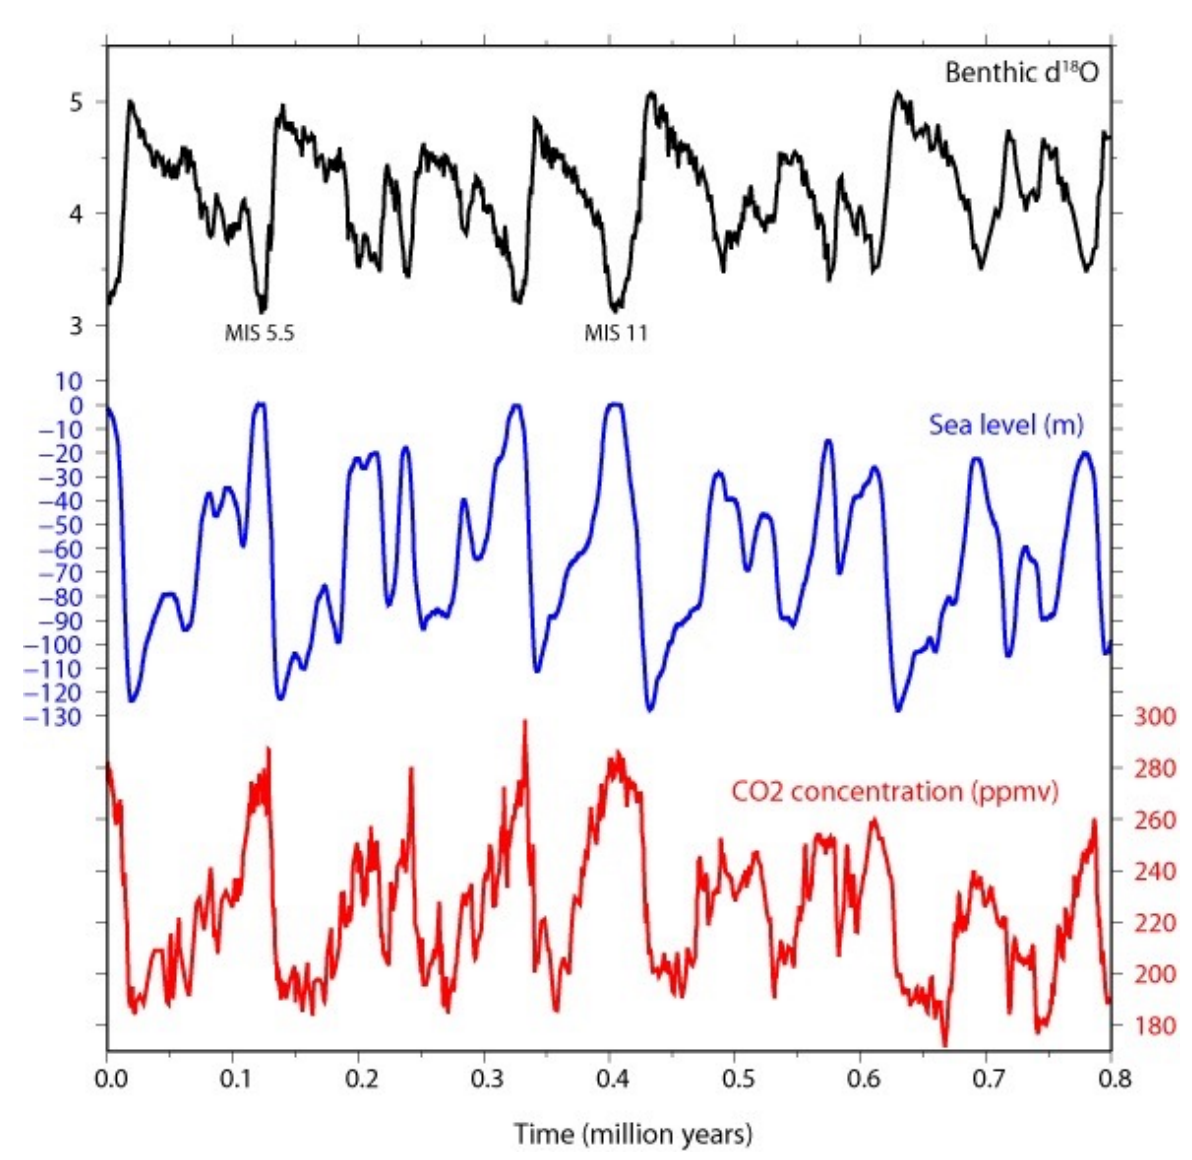
\includegraphics[width=0.5\linewidth]{uploads/graph.png}
    \caption{$\delta$ 18O stack (LR04) from Lisieki and Raymo (2005), sea level estimates (Bintanja et al., 2005) and CO2
concentration from EPICA, Dome C, Antarctica (Lüthi et al., 2008) for the last 0.8 million years.}
\end{figure}
Picco 5e "tirreniano" riconosciuto da certi fossili di fauna senegalese nel Mediterraneo. Passaggio di fasi glaciali e interglaciali sono più netti da fasi integralciali e glaciali in termini di innalzamento di livello del mare (fig.\ref{fig:livelli mare})
\begin{figure}[htpb]
    \centering
    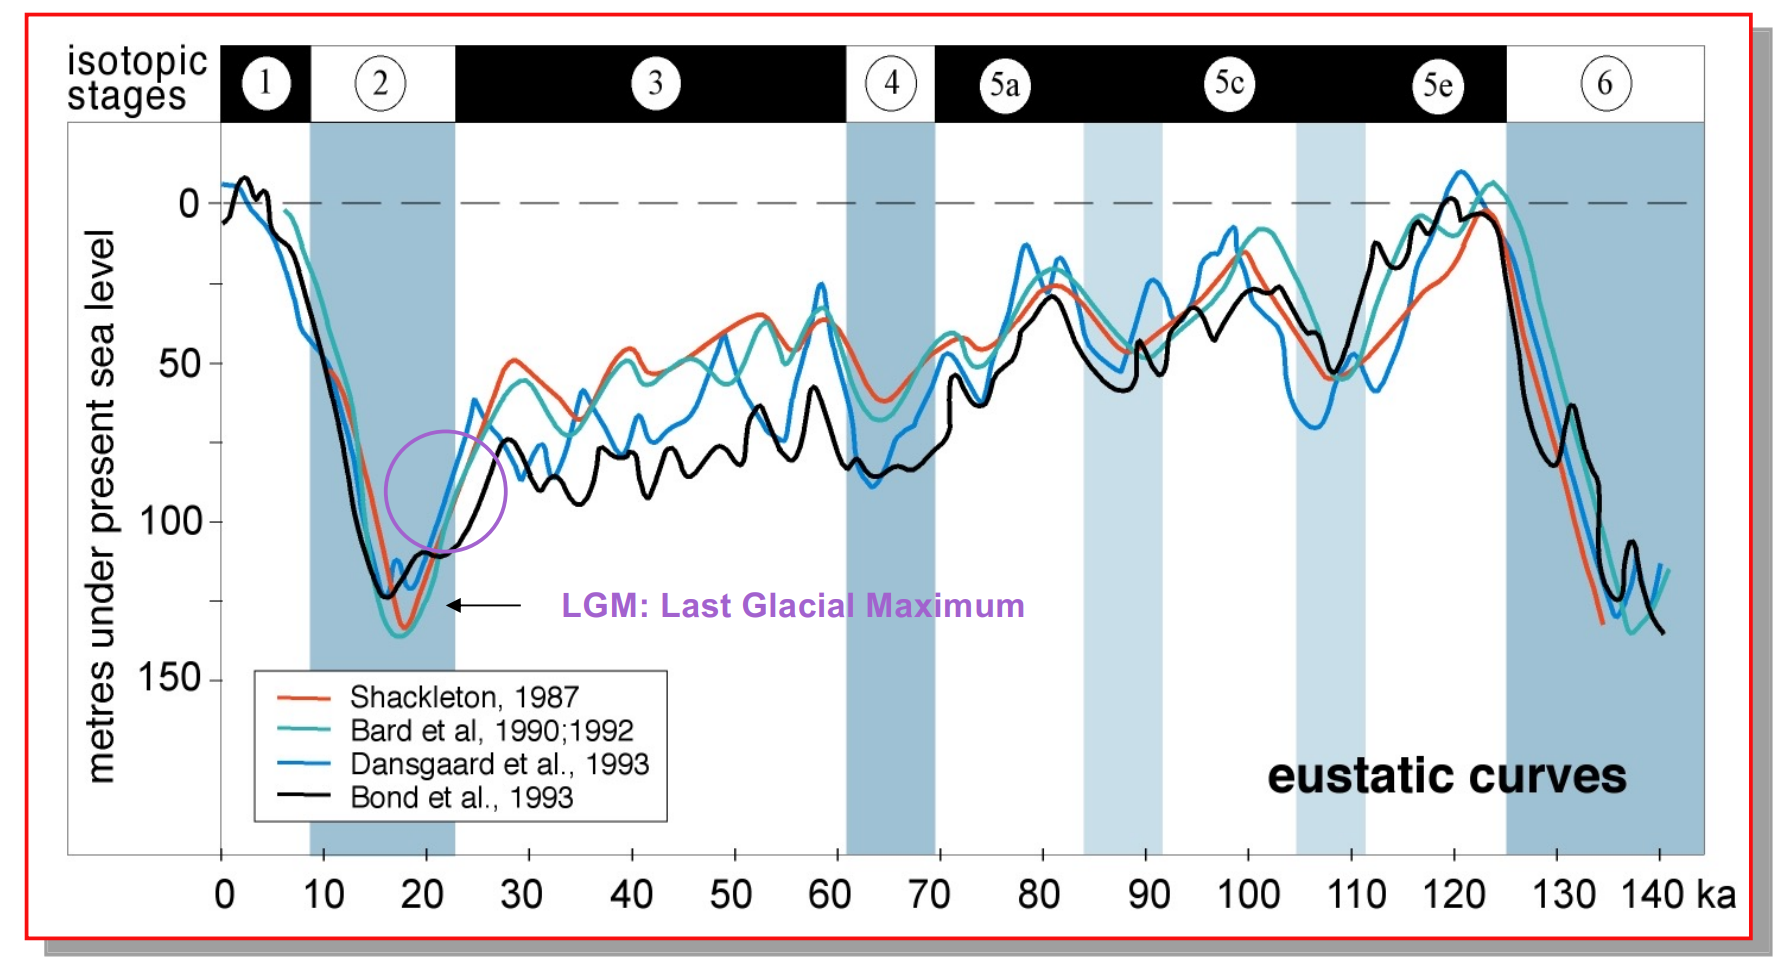
\includegraphics[width=0.5\linewidth]{uploads/livelli.png}
    \caption{Curve riconosciute di innalzamento del livello del mare ed associati stadi isotopici negli ultimi140 ka.}
    \label{fig:livelli mare}
\end{figure}
Scioglimento di calotte glaciali è molto più veloce (meltwater pulses) dando luogo a tassi di risalita inimmaginabili: scioglimento di calotte è più veloce della loro formazione). Nell'ultimo periodo glaciale tutto il mare del Nord era terra emersa, LGM 120m più basso). 
Concetto di rischio e periocolo è legato alla vita umana. Tassi di trasporto dei fiumi (già effetto antropico) negli ultimi migliaia di anni sono stati accelerati dall'uomo. è cambiato il nostro utilizzo del suolo, mettendoci a rischio. 
Olocene, fase di relativa stabilità climatologica. 
\begin{figure}[htpb]
    \centering
    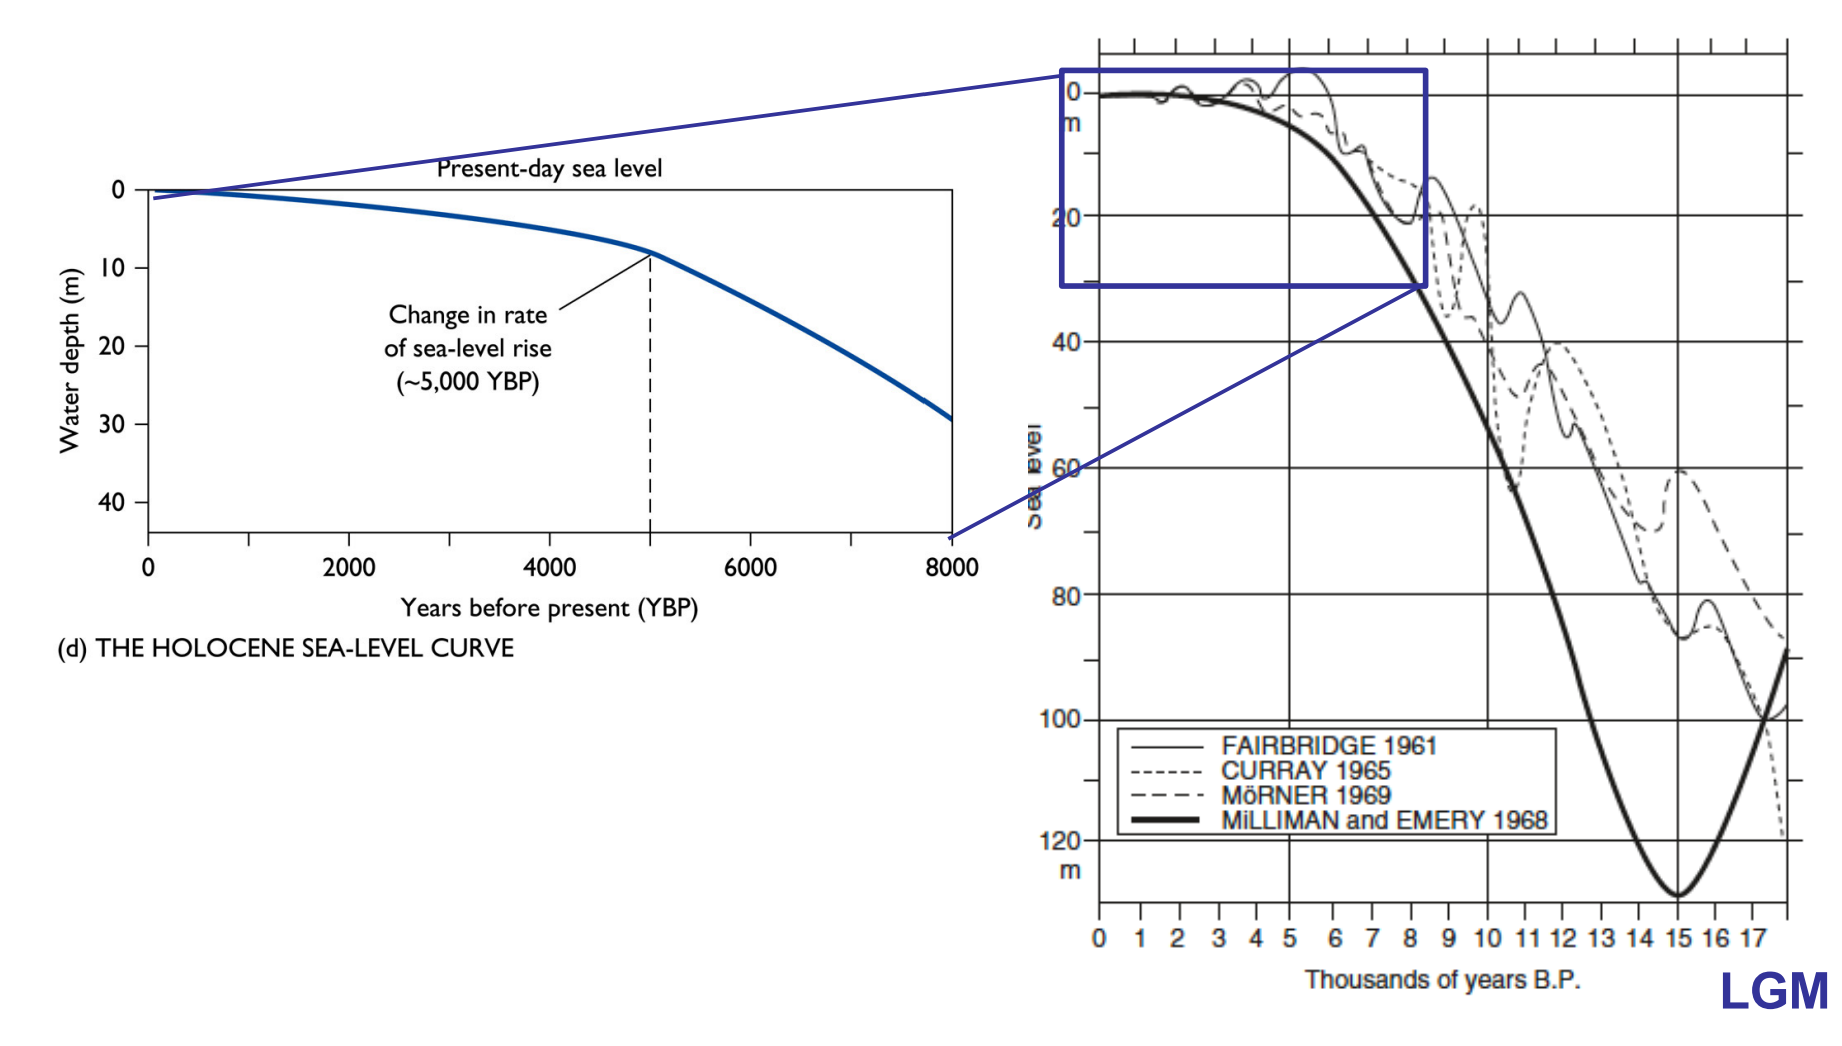
\includegraphics[width=0.5\linewidth]{uploads/innalzamento livelli del mare.png}
    \caption{Tassi medi di innalzamento del livello marino (ultimi 18 ka, da LGM)}
\end{figure}
Certi processi puramente antropogenici aumentano a dismisura in confronto con processi naturali.
\begin{figure}[htpb]
    \centering
    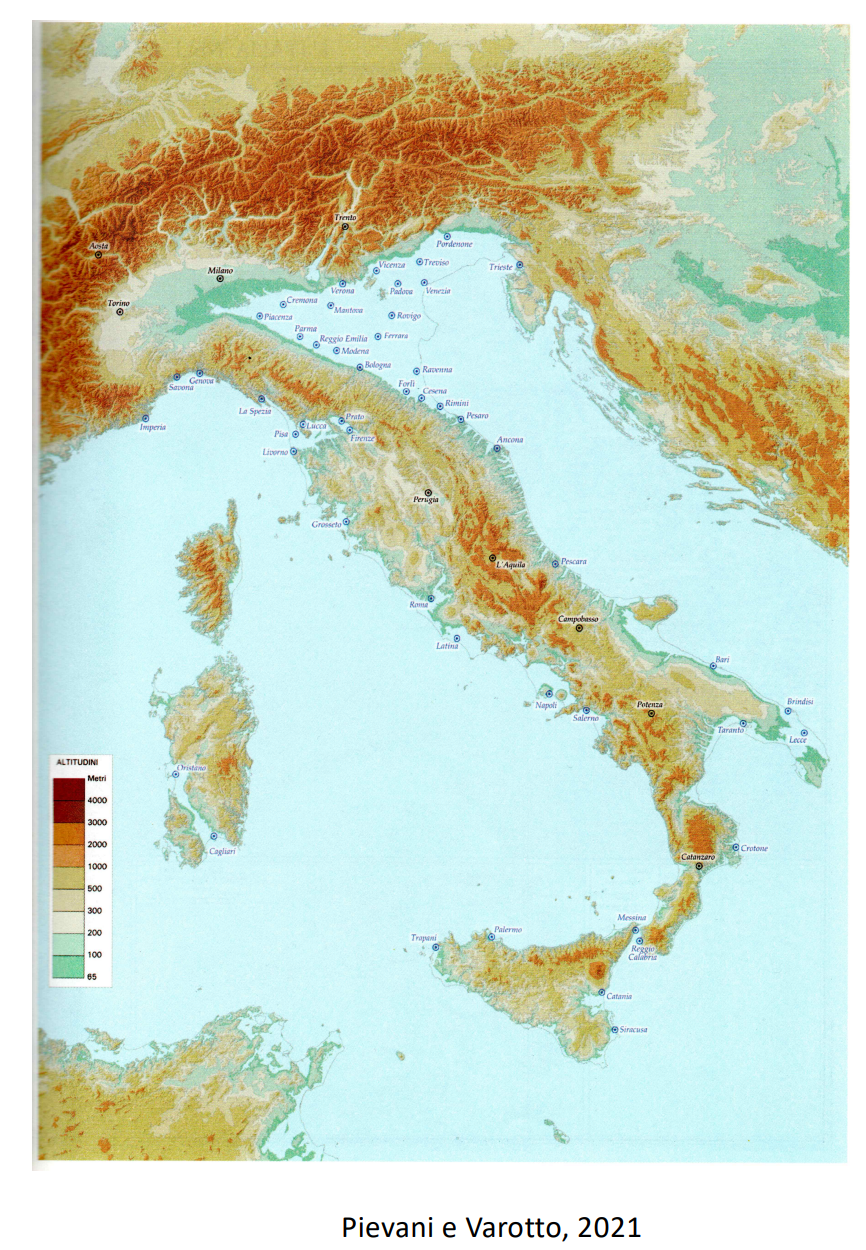
\includegraphics[width=0.5\linewidth]{uploads/italy.png}
    \caption{Italia alla fine del secolo}
\end{figure}
è importante contestualizzare i moderni
cambiamenti climatici rispetto a quelli avvenuti
sul nostro pianeta a scala geologica,
ricostruendo come il sistema climatico ha
risposto e a che tassi (ma potrà rispondere in
modo diverso nel futuro…). Nell’Antropocene ci troviamo in una condizione in cui è l’uomo a modificare
gli equilibri e, contribuendo a cambiare il clima sulla terra, diventa egli stesso
potenzialmente un agente influente anche nella sua evoluzione; questo fenomeno, che non era mai accaduto in tempi così rapidi e con
conseguenze così vaste, ha allontanato il pianeta dal suo «stato olocenico»
di stabilità climatica, verso un’evoluzione futura difficile da modellare.
\section{Rischi geologici}
Rischi vulcanici o sismici sono detti "geofisici" in cui l'umano non ha controllo, rischio idrogeologico e ambientale invece può essere incfluenzata dalla gestione dell'ambiente. Rischio deriva da beni vulnerabili.


Noi ci concentreremo sul rischio delle coste, no other region is more threatened iby natural perils than coasts.
\paragraph{Coasts: the high-risk areas of the world}
\begin{figure}[htpb]
    \centering
    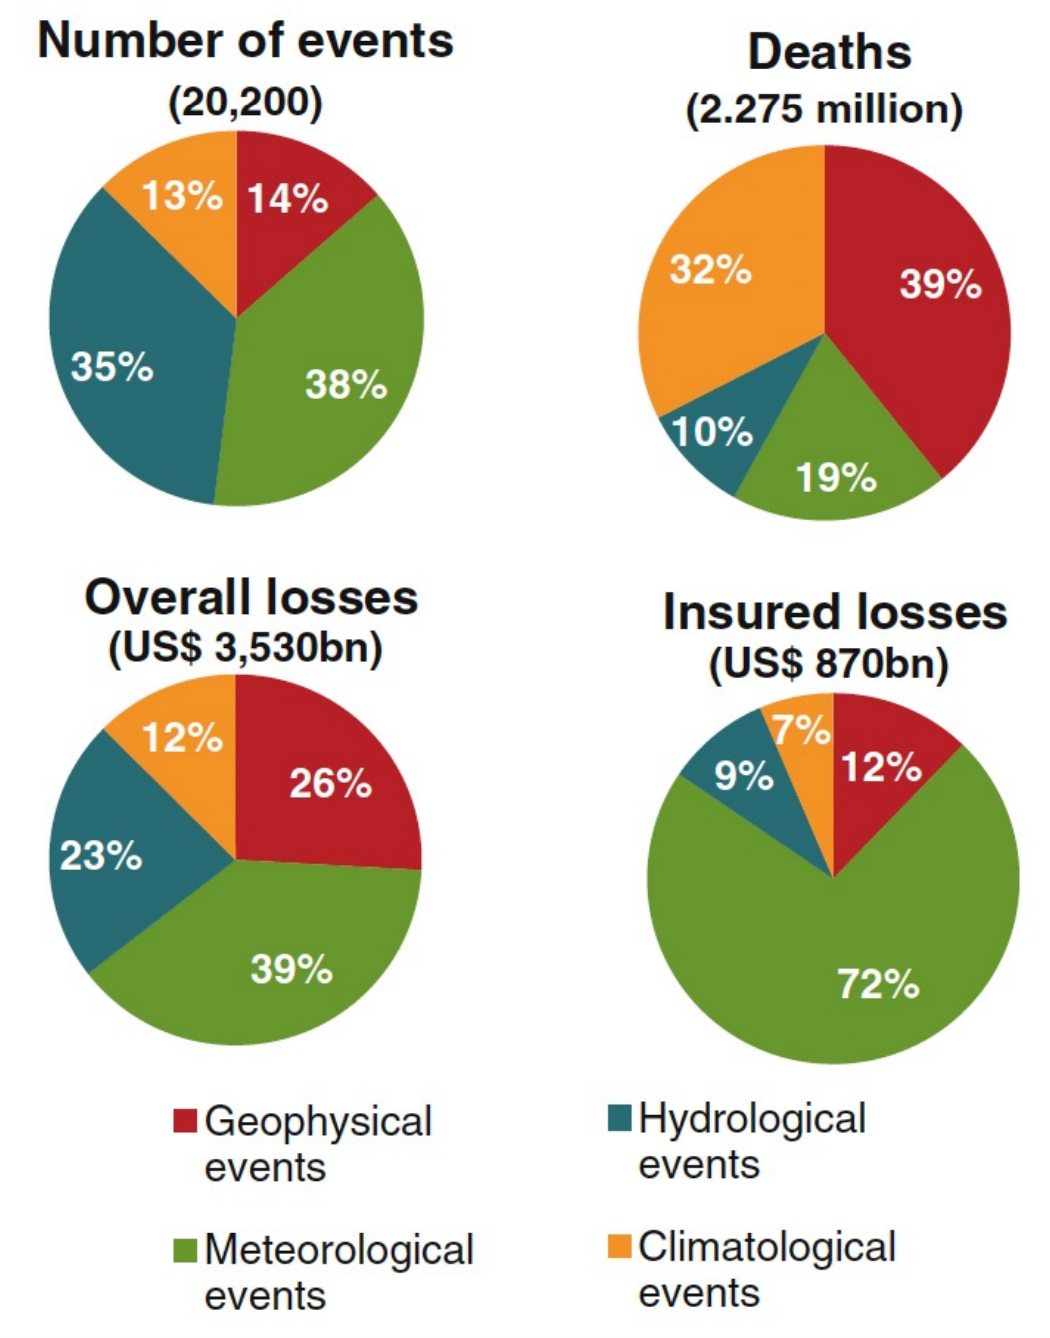
\includegraphics[width=0.5\linewidth]{uploads/paper1.png}
    \caption{Enter Caption}
    \label{fig:enter-label}
\end{figure}

\begin{figure}[htpb]
    \centering
    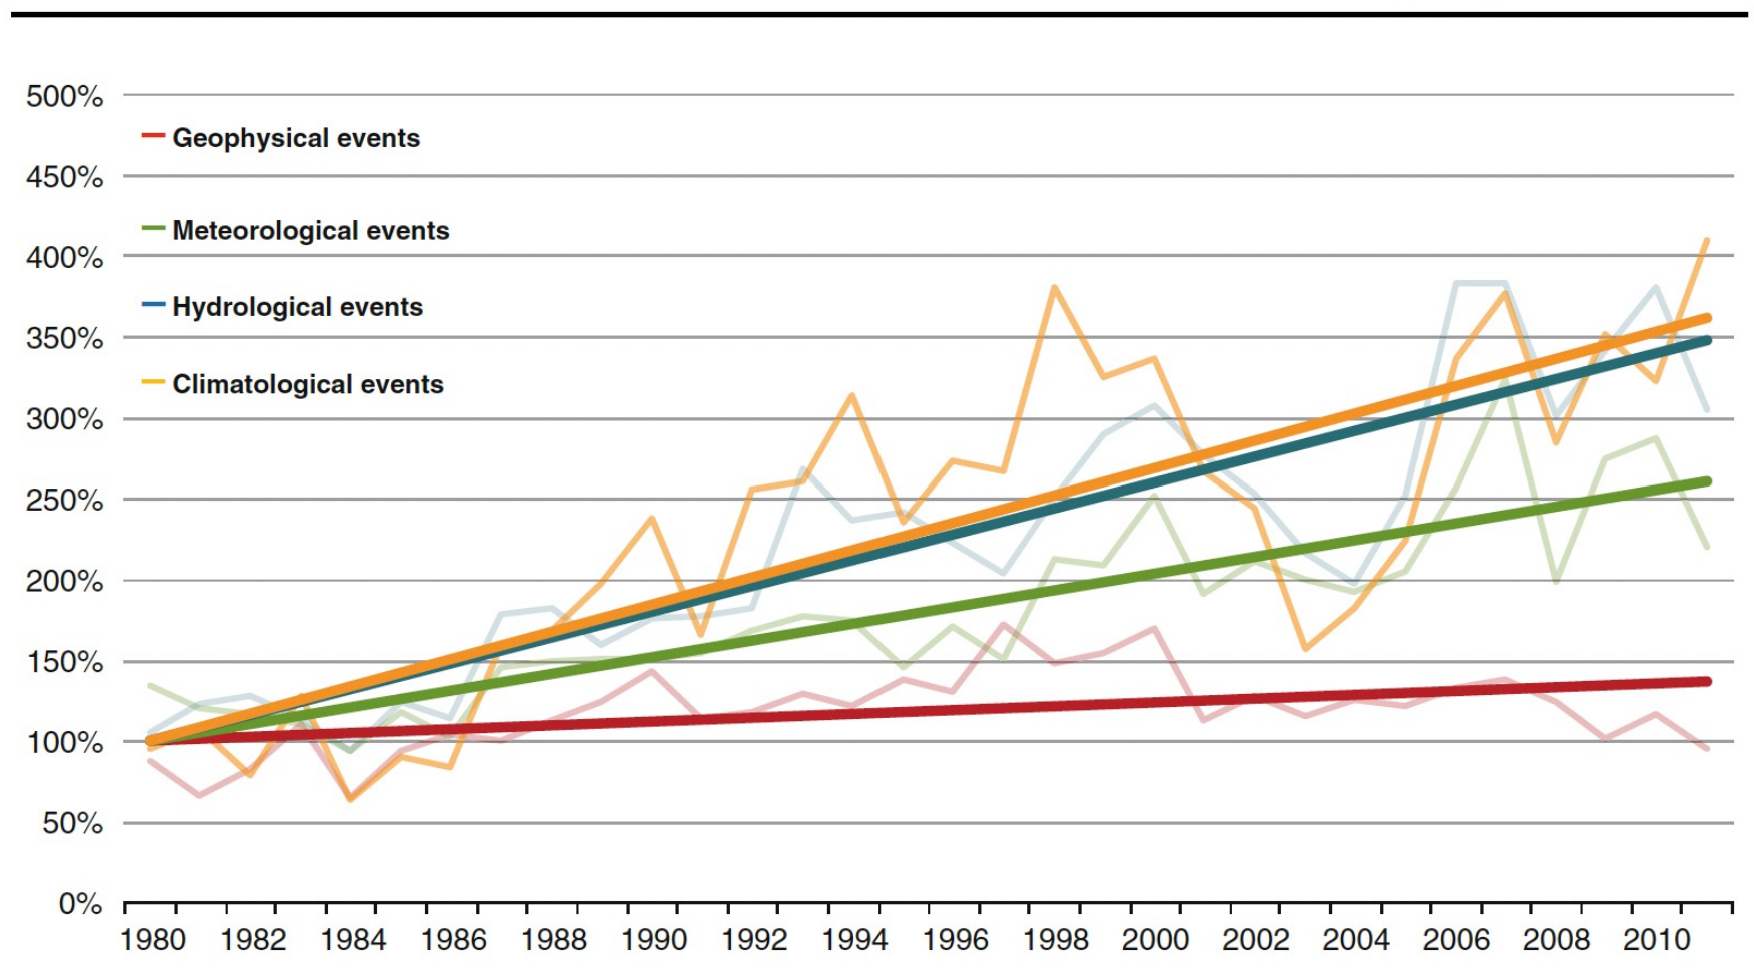
\includegraphics[width=0.5\linewidth]{uploads/paper 2.png}
    \caption{Enter Caption}
    \label{fig:enter-label}
\end{figure}
Le grandi megalopoli sono molto a rischio per la loro quota di beni a disposizione. Il rischio è definito in base ai beni esposti (vulnerabilità umana)!!
\begin{figure}[htpb]
    \centering
    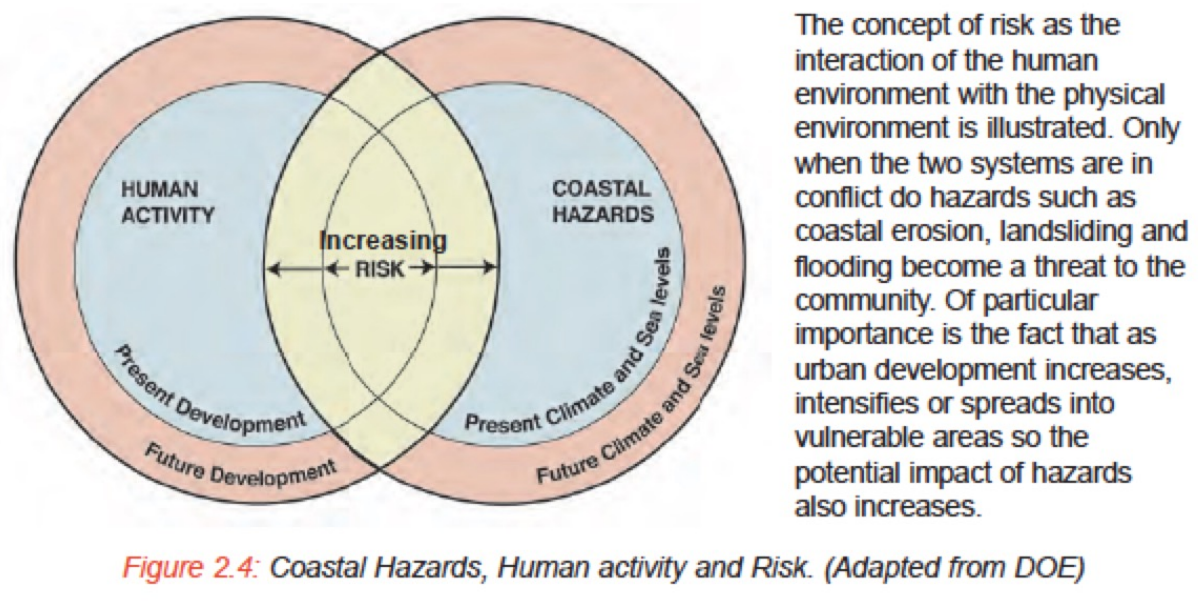
\includegraphics[width=0.5\linewidth]{uploads/rischio.png}
    \caption{Rischio}
\end{figure}
\paragraph{Four Global Catastrophic Risks - A personal view}
\begin{figure}[htpb]
    \centering
    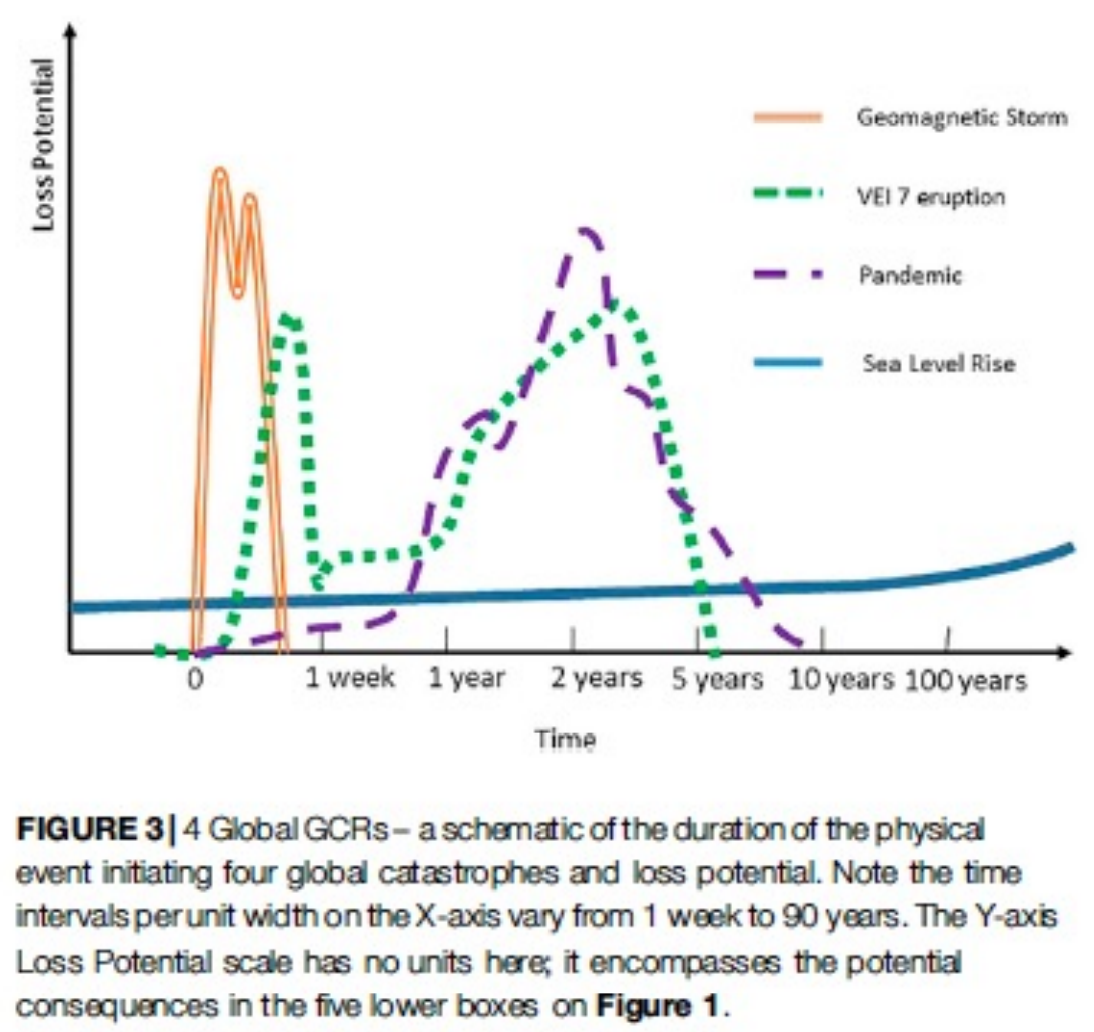
\includegraphics[width=0.5\linewidth]{uploads/catastrophic risk.png}
    \caption{Catastrophic risk}
\end{figure}
\begin{figure}[htpb]
    \centering
    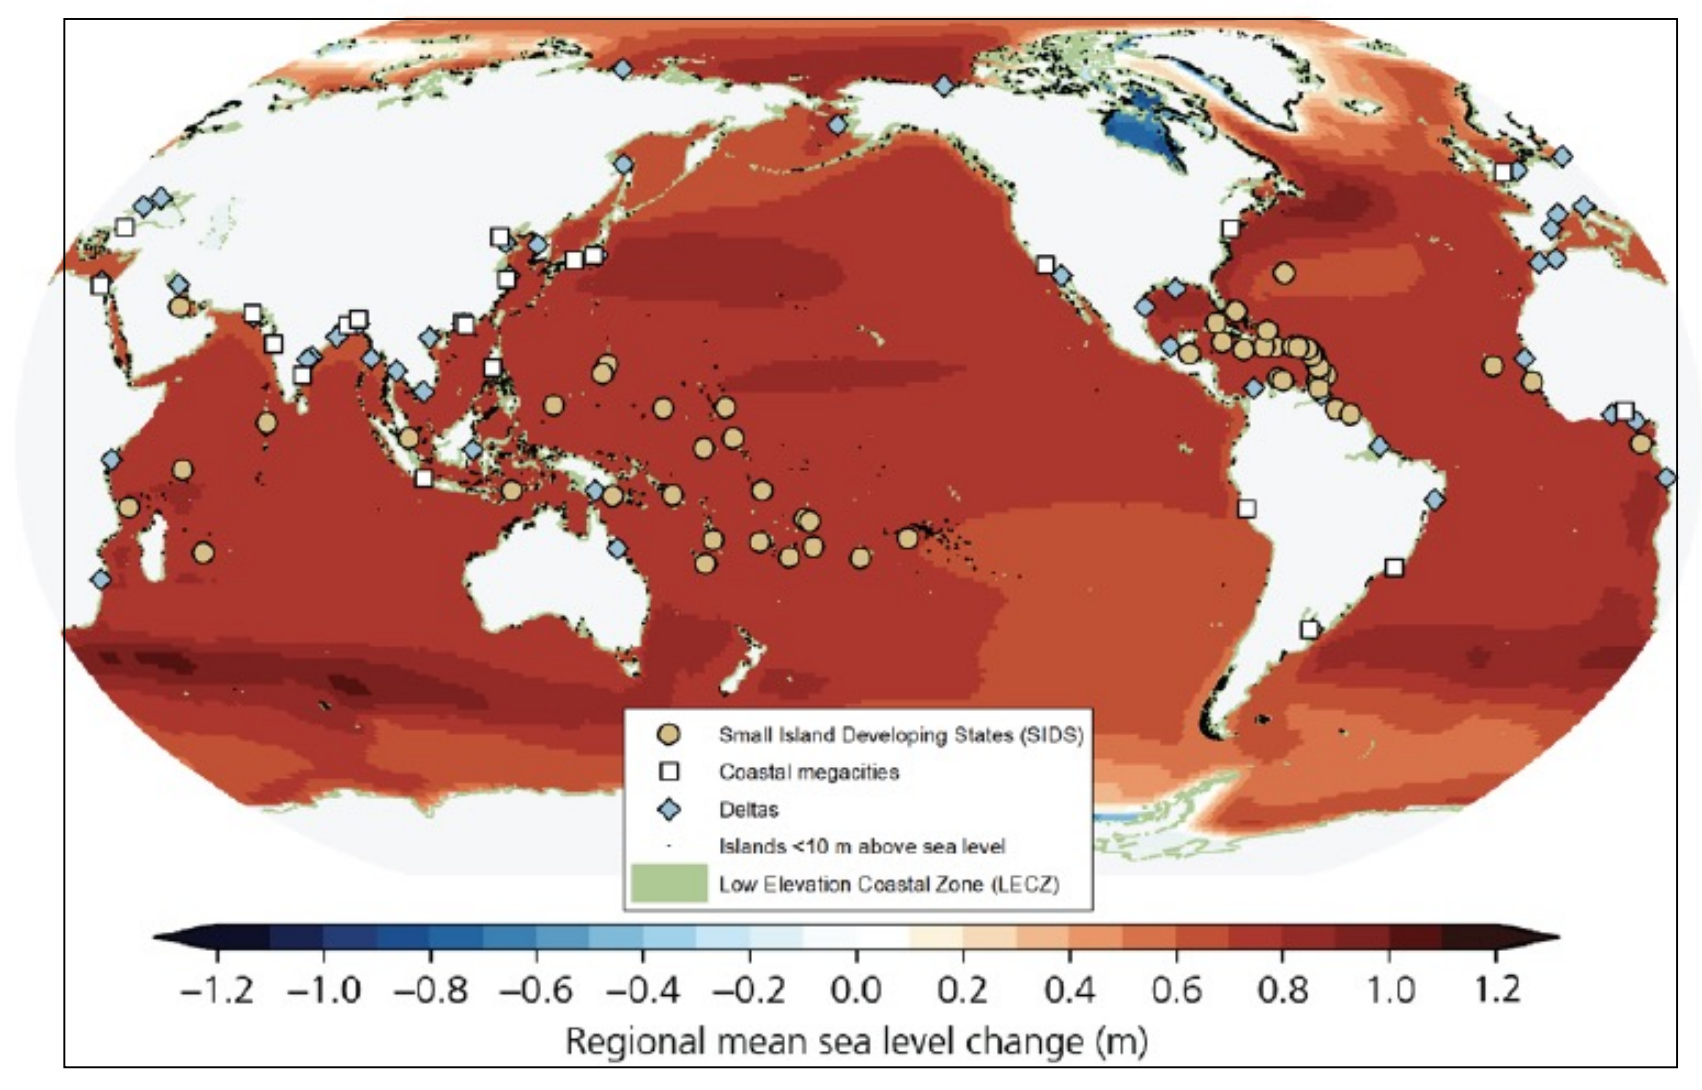
\includegraphics[width=0.5\linewidth]{uploads/SLR impact.png}
    \caption{SLR impact}
\end{figure}
Nel 2019 la popolazione a rischio per l’innalzamento del livello del mare ha raggiunto 190 milioni di persone. Gli effetti impatteranno pesantemente a livello socioeconomico ed ambientale.
